\documentclass[12pt]{extarticle} 
\usepackage{unicode-math}
\usepackage{amsthm,graphicx,xcolor,natbib,enumitem,booktabs,tabularx}
%\usepackage[paperwidth=126mm, paperheight=96mm, top=5mm, bottom=5mm, right=5mm, left=5mm]{geometry}
\usepackage[margin=1cm,footskip=5mm]{geometry}
\pagenumbering{gobble}

\usepackage[BoldFont,SlantFont]{xeCJK}  
\xeCJKsetemboldenfactor{2}
\setCJKmainfont{cwTeX Q Yuan Medium}
\newcommand{\ds}{\displaystyle}
\newcommand{\ie}{\,\Longrightarrow\,}
\newcommand{\ifff}{\,\Longleftrightarrow\,}
\newcommand{\mi}{\mathrm{i}}
\DeclareMathOperator*{\dom}{dom}
\DeclareMathOperator*{\codom}{codom}
\DeclareMathOperator*{\ran}{ran}
\newcommand{\floor}[1]{\lfloor #1 \rfloor}
\newcommand{\ceil}[1]{\lceil #1 \rceil}

% figure --> 圖
\renewcommand{\appendixname}{附錄}
\renewcommand{\figurename}{圖}
\renewcommand{\tablename}{表}
\renewcommand{\refname}{參考文獻}

\usepackage{hyperref}
\hypersetup{
    colorlinks,
    linkcolor={red!50!black},
    citecolor={blue!60!black},
    urlcolor={blue!60!black}
    %urlcolor={blue!80!black}
}

\theoremstyle{definition}
\newtheorem*{dfn}{定義}
\newtheorem*{prp}{性質}
\newtheorem*{thm}{定理}
\newtheorem*{ex}{例}
\newtheorem*{sol}{解}
\newtheorem*{prf}{證}
\newtheorem*{rmk}{註}

%\setenumerate{label=(\roman*),itemsep=1pt,topsep=3pt}
\newcommand{\myline}{\noindent\makebox[\linewidth]{\rule{\paperwidth}{0.4pt}}}
%\newcommand{\myline}{\textcolor[RGB]{220,220,220}{\rule{\linewidth}{1pt}}}

\usepackage{tikz}
\usetikzlibrary{arrows.meta,angles,quotes}

\renewcommand\tabularxcolumn[1]{m{#1}}

\usepackage{fancyhdr}
\fancypagestyle{firststyle} {
   \fancyhf{}
   \fancyfoot[R]{\footnotesize \DTMnow}
   \renewcommand{\headrulewidth}{0pt} 
}
\usepackage{datetime2}
\usepackage{multicol}

\begin{document}
\title{\texorpdfstring{\vspace{-16mm} 第一章\ \ 極限與連續性}{第一章\ \ 極限與連續性}} 
\author{\vspace{-4em}}
\date{\vspace{-4em}}
\maketitle
\thispagestyle{firststyle}

%\newpage

\section*{1.1 直觀極限: 取雙邊接近值}
\vspace{2mm}
\begin{minipage}{0.23\textwidth}
\begin{align*}
  \lim_{x\to 2}x = 2
\end{align*}
\end{minipage}
\qquad
\begin{minipage}{0.77\textwidth}
%\begin{center}
  \begin{tabular}{cccccccc}
    \toprule
    $x$ & 1.9 & 1.99 & 1.999 & $\circ$ & 2.001 & 2.01 & 2.1 \\
    \hline
    \addlinespace[2mm]
    $f(x)$ & 1.9 & 1.99 & 1.999 & $\circ$ & 2.001 & 2.01 & 2.1 \\
    \bottomrule
  \end{tabular}
%\end{center}
\end{minipage}

\vspace{5mm}

\hspace{-7mm}
\begin{minipage}{0.23\textwidth}
\begin{align*}
  \lim_{x\to 2}x^2 = 4
\end{align*}
\end{minipage}
\qquad
\begin{minipage}{0.77\textwidth}
%\begin{center}
  \begin{tabular}{cccccccc}
    \toprule
    $x$ & 1.9 & 1.99 & 1.999 & $\circ$ & 2.001 & 2.01 & 2.1 \\
    \hline
    \addlinespace[2mm]
    $f(x)$ & 3.61 & 3.9601 & 3.996 & $\circ$ & 4.004 & 4.040 & 4.41 \\
    \bottomrule
  \end{tabular}
%\end{center}
\end{minipage}

\vspace{5mm}

%\hspace{-5mm}
\begin{minipage}{0.18\textwidth}
\begin{align*}
  \lim_{x\to 2}\frac{x - 2}{x^2 + x - 6} = 0.2
\end{align*}
\end{minipage}
\qquad
\begin{minipage}{0.85\textwidth}
%\begin{center}
  \begin{tabular}{cccccccc}
    \toprule
    $x$ & 1.9 & 1.99 & 1.999 & $\circ$ & 2.001 & 2.01 & 2.1 \\
    \hline
    \addlinespace[2mm]
    $f(x)$ & 0.20408 & 0.20040 &0.20004 & $\circ$ & 0.19996 & 0.19960 & 0.19608 \\
    \bottomrule
  \end{tabular}
%\end{center}
\end{minipage}

\vspace{2mm}

%\begin{align*}
%  f(x) = \begin{cases}x & x < 2 \\ -1 & x = 2 \\ x + 3 & x > 2\end{cases} \\
%  \lim_{x\to 2}f(x) = \text{DNE}
%\end{align*}
%
%\begin{center}
%  \begin{tabular}{cccccccc}
%    \toprule
%    $x$ & 1.9 & 1.99 & 1.999 & $\circ$ & 2.001 & 2.01 & 2.1 \\
%    \hline
%    $f(x)$ & 1.9 & 1.99 & 1.999 & $\circ$ & 5.001 & 5.01 & 5.1 \\
%    \bottomrule
%  \end{tabular}
%\end{center}

\section*{1.2 單側極限, 無限遠極限, 無窮極限}

\subsection*{單側極限 (One-Sided Limits) }

\vspace{-3mm}
\hspace{1cm}
\begin{minipage}{0.4\textwidth}
  \begin{align*}
    \lim_{x\to2-}g(x) = 3,\qquad\lim_{x\to5-}g(x) = 2 \\
    \lim_{x\to2+}g(x) = 1,\qquad\lim_{x\to5+}g(x) = 2 \\
    \lim_{x\to2}g(x) = \text{DNE},\qquad\lim_{x\to5}g(x) = 2
  \end{align*}
\end{minipage}
\begin{minipage}{0.6\textwidth}
  \begin{center}
    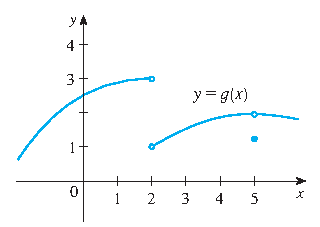
\includegraphics[scale=1.,page=1]{fig/g.pdf}
  \end{center}
\end{minipage}

\begin{ex}
  $\ds g(x) = \begin{cases}\sqrt{x - 4} & \text{若 } x > 4 \\ 8 - 2x & \text{若 } x < 4 \end{cases}$, $\ds\lim_{x\to 4}g(x) = 0$. 
\end{ex}

\begin{ex}
  $\ds f(x) = \sqrt{4 - x^2}$, $\ds\lim_{x\to(-2)+}f(x) = 0$, $\ds\lim_{x\to2+}f(x) = \text{DNE}$, $\ds\lim_{x\to2-}f(x) = 0$. 
\end{ex}

\begin{ex}
  \setlength{\columnsep}{-30mm}
  \begin{multicols}{3}
    \begin{itemize}\setlength\itemsep{0em}
      \item $\ds\lim_{x\to0}|x| = 0$
      \item $\ds\lim_{x\to0}\frac{|x|}{x} = \text{DNE}$
      \item $\ds\lim_{x\to3+}\floor{x} = 3$, $\ds\lim_{x\to3-}\floor{x} = 2$, $\ds\lim_{x\to\pi}\floor{x} = 3$. 
    \end{itemize}
  \end{multicols}
\end{ex}

\begin{thm}
  若 $F\in\mathbb{R}$, $\ds\lim_{x\to a}f(x) = F$ $\ifff$ $\ds\lim_{x\to a-} f(x) = \ds\lim_{x\to a+} f(x) = F$. 
\end{thm}

%\begin{ex}
%  給定 $n\in\mathbb{Z}$, $\ds\lim_{x\to n}\floor{x - \floor{x - 1}} = 1$. 
%\end{ex}
%
%\begin{sol}
%  \begin{itemize}\setlength\itemsep{0em}
%    \item[]
%    \item 當 $\ds x = n + \varepsilon$, $\ds 0\leqslant\varepsilon\ll 1$, $\ds\floor{x - \floor{x - 1}} = \floor{(n + \varepsilon) - \floor{(n - 1) + \varepsilon}} = \floor{(n + \varepsilon) - (n - 1)} = \floor{1 + \varepsilon} = 1$, 則 $\ds\lim_{x\to n+}\floor{x - \floor{x - 1}} = 1$. 
%    \item 當 $\ds x = n - \varepsilon$, $\ds 0\leqslant\varepsilon\ll 1$, $\ds\floor{x - \floor{x - 1}} = \floor{(n - \varepsilon) - \floor{(n - 1) - \varepsilon}} = \floor{(n - \varepsilon) - (n - 2)} = \floor{2 - \varepsilon} = 1$, 則 $\ds\lim_{x\to n-}\floor{x - \floor{x - 1}} = 1$. 
%    \item 由上定理 $\ds\lim_{x\to n}\floor{x - \floor{x - 1}} = 1$. 
%  \end{itemize}
%\end{sol}

\subsection*{無限遠極限 (Limits at Infinity) }
\begin{ex}
  \begin{multicols}{2}
    \begin{itemize}\setlength\itemsep{0em}
      \item $\ds\lim_{x\to\infty}\frac{1}{x^\alpha} = 0$, $\alpha > 0$; $\ds\lim_{x\to-\infty}\frac{1}{x^N} = 0$, $\forall\,N\in\mathbb{N}$
      \item $\ds\lim_{x\to\infty}\tan^{-1} x = \frac{\pi}{2}$, $\ds\lim_{x\to-\infty}\tan^{-1} x = -\frac{\pi}{2}$
      \item $\ds\lim_{x\to\infty}a^x = \infty$, $\ds\lim_{x\to-\infty}a^x = 0$, $\ds\lim_{x\to0-}a^{\frac{1}{x}} = 0$, $\forall\,a > 1$. 
    \end{itemize}
  \end{multicols}
\end{ex}

\subsection*{無窮極限 (Infinite Limits) }
\begin{ex}
  \setlength{\columnsep}{-20mm}
  \begin{multicols}{5}
    \begin{itemize}\setlength\itemsep{0em}
      \item $\ds\lim_{x\to0+}\frac{1}{x} = \infty$
      \item $\ds\lim_{x\to0-}\frac{1}{x} = -\infty$
      \item $\ds\lim_{x\to0}\frac{1}{x} = \text{DNE}$
      \item $\ds\lim_{x\to0}\frac{1}{x^2} = \infty$
      \item $\ds\lim_{x\to\frac{\pi}{2}-}\tan x = \infty$
    \end{itemize}
  \end{multicols}
\end{ex}

\section*{1.3 極限運算}

\begin{prp}
  若函數 $f$ 為多項式, 指數, 對數, 三角, 或反三角函數, 則 $\ds\lim_{x\to a}f(x) = f(a)$, $\forall\,a\in\dom f$.
\end{prp}

\begin{ex}
  %\setlength{\columnsep}{-30mm}
  \begin{multicols}{3}
    \begin{itemize}\setlength\itemsep{0em}
      \item $\ds\lim_{x\to\pi} \frac{1}{x^2} = \frac{1}{\pi^2}$
      \item $\ds\lim_{x\to\pi} x^{\pi} = {\pi}^\pi$
      \item $\ds\lim_{x\to -3} \Big(\frac{1}{3}\Big)^{x} = 27$
      \item $\ds\lim_{x\to -5}\cos x = \cos(-5) = \cos 5$
      \item $\ds\lim_{x\to 1}\tan^{-1} x = \frac{\pi}{4}$
      \item $\ds\lim_{x\to 5}\log_2 x = \log_2 5$% = \lim_{x\to 5+} \log_2 x = \lim_{x\to 5-} \log_2 x$
    \end{itemize}
  \end{multicols}
\end{ex}

\begin{thm}[極限四則運算]
  若 $\ds\lim_{x\to a}f(x) = F$, $\ds\lim_{x\to a}g(x) = G$, 則
  \begin{multicols}{2}
    \begin{enumerate}\setlength\itemsep{0em}
      \item $\ds\lim_{x\to a} c = c$, $\ds\lim_{x\to a} x = a$
      \item $\ds\lim_{x\to a} k\,f(x) = k\,F$ 
      \item $\ds\lim_{x\to a} \big(f(x)\pm g(x)\big) = F\pm G$ 
      \item $\ds\lim_{x\to a} \big(f(x)\cdot g(x)\big) = F\cdot G$ 
      \item $\ds\lim_{x\to a} \frac{f(x)}{g(x)} = \frac{F}{G}$, 若 $G\ne 0$
      \item $\ds\lim_{x\to a} \big(f(x)\big)^\alpha = F^\alpha$, 若 $\alpha\in\mathbb{Q}\,\wedge\,F > 0$
    \end{enumerate}
  \end{multicols}
  當 $F$, $G$ 存在 (非為無窮) , 此定理敘述對「單側極限」及「無限遠極限」均成立. 
\end{thm}

\begin{ex}
  \begin{multicols}{2}
    \begin{itemize}\setlength\itemsep{0em}
      \item $\ds\lim_{t\to-1}\frac{t - 2}{t + 3} = \frac{\lim_{t\to-1} t - 2}{\lim_{t\to-1}t + 3} = \frac{-3}{2}$
      \item $\ds\lim_{t\to-3}\frac{1 - t}{\cos t} = \frac{\lim_{t\to-3} 1 - t}{\lim_{t\to-3}\cos t} = \frac{4}{\cos{3}}$
    \end{itemize}
  \end{multicols}
\end{ex}

\begin{ex}
  \begin{itemize}\setlength\itemsep{0em}
    \item[]
    \item $\ds\lim_{h\to0}\frac{(2 + h)^2 - 4}{2 h} = \lim_{h\to0}\frac{h^2 + 4h + 4 - 4}{2 h} = \lim_{h\to0}\frac{h^2 + 4h}{2 h} =\lim_{h\to0}\frac{h + 4}{2} = 2$
    \item $\ds\lim_{x\to4}\frac{x^2 - 4x}{x^2 - 16} = \lim_{x\to4}\frac{x(x - 4)}{(x - 4)(x + 4)} = \lim_{x\to4}\frac{x}{x + 4} = \frac{1}{2}$
    \item $\ds\lim_{x\to 2}\frac{x - 2}{x^2 + x - 6} = \lim_{x\to 2}\frac{x - 2}{(x - 2)(x + 3)} = \lim_{x\to2}\frac{1}{x + 3} = \frac{1}{5}$
  \end{itemize}
\end{ex}

\myline

\begin{ex}  
  \begin{multicols}{2}
    \begin{enumerate}\setlength\itemsep{0em}
      \item $\ds\lim_{x\to-1}\frac{\sqrt{x^2 + 8} - 3}{x + 1}$. 
      \item $\ds\lim_{x\to3}\frac{\sqrt{x - 2} - \sqrt{4 - x}}{x - 3}$.
    \end{enumerate}
  \end{multicols}
\end{ex}

\begin{sol}
  \begin{enumerate}\setlength\itemsep{0em}
    \item[]
    \item $\ds\lim_{x\to-1}\frac{\sqrt{x^2 + 8} - 3}{x + 1} = \lim_{x\to-1}\frac{1}{x + 1}\frac{(x^2 + 8) - 3^2}{\sqrt{x^2 + 8} + 3} = \lim_{x\to-1}\frac{1}{x + 1}\frac{x^2 - 1}{\sqrt{x^2 + 8} + 3} \\= \lim_{x\to-1}\frac{1}{x + 1}\frac{(x + 1)(x - 1)}{\sqrt{x^2 + 8} + 3} =\lim_{x\to-1}\frac{x - 1}{\sqrt{x^2 + 8} + 3} = \frac{-2}{\sqrt{1 + 8} + 3} = -\frac{1}{3}$. 
    \item $\ds\lim_{x\to3}\frac{\sqrt{x - 2} - \sqrt{4 - x}}{x - 3} = \lim_{x\to3}\frac{1}{x - 3}\frac{(x - 2) - (4 - x)}{\sqrt{x - 2} + \sqrt{4 - x}} = \lim_{x\to3}\frac{1}{x - 3}\frac{2 x - 6}{\sqrt{x - 2} + \sqrt{4 - x}} \\= \lim_{x\to3}2\frac{1}{\sqrt{x - 2} + \sqrt{4 - x}} = \frac{2}{\sqrt{1} + \sqrt{1}} = 1$. 
  \end{enumerate}
\end{sol}

\begin{ex}
  $\ds\lim_{x\to\infty}\frac{5x^2 + 8x - 3}{3x^2 + 2} = \lim_{x\to\infty}\frac{5 + \frac{8}{x} - \frac{3}{x^2}}{3 + \frac{2}{x^2}} = \frac{5 + 0 + 0}{3 + 0} = \frac{5}{3} = \lim_{x\to-\infty}\frac{5x^2 + 8x - 3}{3x^2 + 2}$. 
\end{ex}

\begin{ex}
  求 $\ds\lim_{x\to\infty}\big(\sqrt{x^2 + 5x} - \sqrt{x^2 - x}\big)$. 
\end{ex}

\begin{sol}
  $\ds\lim_{x\to\infty}\big(\sqrt{x^2 + 5x} - \sqrt{x^2 - x}\big) = \lim_{x\to\infty}\frac{(x^2 + 5x) - (x^2 - x)}{\sqrt{x^2 + 5x} + \sqrt{x^2 - x}} = \lim_{x\to\infty}\frac{6x}{\sqrt{x^2 + 5x} + \sqrt{x^2 - x}} \\= \lim_{x\to\infty}\frac{6 x}{\sqrt{x^2\big(1 + \frac{5}{x}\big)} + \sqrt{x^2\big(1 - \frac{1}{x}\big)}} = \lim_{x\to\infty}\frac{6 x}{|x|\sqrt{1 + \frac{5}{x}} + |x|\sqrt{1 - \frac{1}{x}}} = \lim_{x\to\infty}\frac{6 x}{x\sqrt{1 + \frac{5}{x}} + x\sqrt{1 - \frac{1}{x}}} \\= \lim_{x\to\infty}\frac{6}{\sqrt{1 + \frac{5}{x}} + \sqrt{1 - \frac{1}{x}}} = \frac{6}{\sqrt{1 + 0} + \sqrt{1 - 0}} = 3$
\end{sol}

\begin{ex}
  求 $\ds\lim_{x\to-\infty}\frac{3x}{\sqrt{4x^2 + x} - 2x}$. 
\end{ex}

\begin{sol}
  \begin{itemize}\setlength\itemsep{0em}
    \item[]
    \item $\ds\lim_{x\to-\infty}\frac{3x}{\sqrt{4x^2 + x} - 2x} = \lim_{x\to-\infty}\frac{3x}{\sqrt{x^2(4 + \frac{1}{x})} - 2x} = \lim_{x\to-\infty}\frac{3x}{|x|\sqrt{4 + \frac{1}{x}} - 2x} = \lim_{x\to-\infty}\frac{3x}{-x\sqrt{4 + \frac{1}{x}} - 2x} = \lim_{x\to-\infty}\frac{3}{-\sqrt{4 + \frac{1}{x}} - 2} = -\frac{3}{4}$. 
    \item 另解: 變數變換 $y = -x\ie x=-y$: $\ds\lim_{x\to-\infty}\frac{3x}{\sqrt{4x^2 + x} - 2x} = \lim_{y\to\infty}\frac{-3y}{\sqrt{4y^2 - y} + 2y} \\= \lim_{y\to\infty}\frac{-3y}{\sqrt{y^2\big(4 - \frac{1}{y}\big)} + 2y} = \lim_{y\to\infty}\frac{-3y}{|y|\sqrt{4 - \frac{1}{y}} + 2y} = \lim_{y\to\infty}\frac{-3y}{y\sqrt{4 - \frac{1}{y}} + 2y} =\lim_{y\to\infty}\frac{-3}{\sqrt{4 - \frac{1}{y}} + 2} = -\frac{3}{4}$. 
  \end{itemize}
\end{sol}

\begin{thm}[夾擠 (squeeze) 定理; 三明治定理]
  若 $g(x)\leqslant f(x)\leqslant h(x)$ $\forall\,x\in[a, b]$, $c\in[a, b]$ 且 $\ds\lim_{x\to c}g(x) = \lim_{x\to c}h(x) = L$, 則 $\ds\lim_{x\to c} f(x) = L$. 
\end{thm}

\begin{ex}
  求 $\ds\lim_{x\to 0}x\sin^2\frac{1}{x}$. 
\end{ex}

\begin{sol}
  若 $x\ne 0$, $\ds 0\leqslant\sin^2\frac{1}{x}\leqslant 1$, 則 $\ds-|x|\leqslant x\sin^2\frac{1}{x}\leqslant|x|$. 又 $\ds\lim_{x\to 0}(-|x|) = \lim_{x\to 0}|x| = 0$, 由夾擠定理 $\ds\lim_{x\to 0}x\sin^2\frac{1}{x} = 0$. 
\end{sol}

\section*{1.4 連續性}

\begin{dfn} 給定 $f$, $a\in\dom f$. 
  \begin{itemize}\setlength\itemsep{0em}
    \item 若 $\ds\lim_{x\to a} f(x)$ 存在且 $\ds f(a)=\lim_{x\to a}f(x)$, 則稱 $f$ 在 $a$ \emph{連續}.  
    \item 若 $\ds\lim_{x\to a+} f(x)$ 存在且 $\ds f(a)=\lim_{x\to a+}f(x)$, 則稱 $f$ 在 $a$ \emph{左連續}.  
    \item 若 $\ds\lim_{x\to a-} f(x)$ 存在且 $\ds f(a)=\lim_{x\to a-}f(x)$, 則稱 $f$ 在 $a$ \emph{右連續}.  
  \end{itemize}
  $f(x)$ 在 $a$ 連續 $\ifff$ $\ds\lim_{x\to a}f(x) = f\big(\lim_{x\to a}x\big) = f(a)$, 亦即(極限值) $=$ (函數值).
\end{dfn}

\begin{dfn}[端點連續性]
  給定 $f$, $\dom f = [a, b]$.  
  \begin{multicols}{2}
    \begin{itemize}\setlength\itemsep{0em}
      \item 若 $f$ 在 $b$ 左連續, 則稱 $f$ 在 $b$ 連續.  
      \item 若 $f$ 在 $a$ 右連續, 則稱 $f$ 在 $a$ 連續.  
    \end{itemize}
  \end{multicols}
\end{dfn}

\begin{dfn}[連續函數] 
  \begin{itemize}\setlength\itemsep{0em}
    \item[]
    \item 若 $f$ 在區間 $I$ 之每一點均連續, 則稱 $f$ 在 $I$ 連續.  
    \item 若 $f$ 在 $\dom f$ 之每一點均連續, 則稱 $f$ 為\emph{連續函數}.  
  \end{itemize}
\end{dfn}

\begin{thm}[五則運算仍連續]
  \begin{itemize}\setlength\itemsep{0em}
    \item[] 
    \item 若 $f$, $g$ 在 $a$ 連續, 則 $f\pm g$, $f\cdot g$, $k f$, $f^\alpha$, $\ds\frac{f}{g}$ (若 $g(a)\ne 0$) 均在 $a$ 連續. 
    \item 若 $f$ 在 $a$ 連續, 且 $g$ 在 $f(a)$ 連續, 則 $g\circ f$ 在 $a$ 連續. 
  \end{itemize}
\end{thm}

\begin{prp}
  多項式, 指數, 對數, 三角, 反三角函數及其五則運算在其定義域內均為連續函數. 
\end{prp}

\begin{ex}
  若 $\ds f(x) = \begin{cases}x + 2 & \text{當 }\; x < a \\ x^2 & \text{當 }\; x\geqslant a\end{cases}$ 為連續函數, 求 $a$. 
\end{ex}

\begin{sol}
  若 $f$ 為連續函數, 則 $f$ 在 $a$ 連續 $\ds\ie \lim_{x\to a-}f(x) = \lim_{x\to a+} f(x) \ie a + 2 = a^2 \ie a = -1\,\vee\, a = 2$. 
\end{sol}

\begin{ex}
  若 $\ds f(x) = \begin{cases}\frac{x^2 - 4}{x - 2} & \text{當 }\; x < 2 \\ a x^2 - b x + 3 & \text{當 }\; 2 \leqslant x < 3 \\ 2 x - a + b & \text{當 }\; x \geqslant 3 \end{cases}$ 為連續函數, 求 $a$, $b$. 
\end{ex}

\begin{sol}
  若 $f$ 為連續函數, 則 $f$ 在 $2$, $3$ 均連續 $\ds\ie \big(\lim_{x\to 2-}f(x) = \lim_{x\to 2+} f(x)\big) \,\wedge\, \big(\lim_{x\to 3-}f(x) = \lim_{x\to 3+} f(x)\big)\ie (4 = 4a - 2b + 3)\,\wedge\, (9a - 3b + 3 = 6 - a + b)\ie a = \frac{1}{2},\,\,b = \frac{1}{2}$. 
\end{sol}

\begin{thm}[Bolzano 定理; 勘根定理]
  若 $f$ 在 $[a, b]$ 連續且 $f(a)\cdot f(b) < 0$, 則存在 $c\in(a, b)$ 使得 $f(c) = 0$.   
\end{thm}

\begin{thm}[中間值定理]
  若 $f$ 在 $[a, b]$ 連續, 則對任意介於 $f(a)$ 與 $f(b)$ 之間的數 $d$, 存在 $c\in[a, b]$ 使得 $f(c) = d$.   
\end{thm}

\begin{rmk}%\leavevmode
  \begin{itemize}\setlength\itemsep{0em}
    \item[]
    \item 中間值定理不適用於不連續函數: 取 $\ds f(x) = \begin{cases}x + 2 & -1 < x \leqslant 1 \\ x & -2\leqslant x\leqslant -1\end{cases}$, 則 $f(-2) < 0$, $f(1) > 0$, 但 $f(x) = 0$ 無解. 
    \item $\ds f(x) = \begin{cases}x\sin\frac{1}{x}& x \ne 0 \\ 0 & x = 0\end{cases}$, 則存在無限多 $x\in[-\frac{2}{3\pi},\,\frac{2}{\pi}]$ 使 $f(x) = 0$. 
  \end{itemize}
\end{rmk}

\begin{ex}
  證明 $4x^3 - 6x^2 + 3x - 2 = 0$ 在 $1$, $2$ 間有實根. 
\end{ex}

\begin{sol}
  令 $f(x) = 4x^3 - 6x^2 + 3x - 2$. $f$ 為連續函數且 $f(1) < 0$, $f(2) > 0$, 由 Bolzano 定理知存在 $c\in(1, 2)$ 使得 $f(c) = 0$, 亦即 $4x^3 - 6x^2 + 3x - 2 = 0$ 在 $1$, $2$ 間有實根. 
\end{sol}

\begin{ex}
  證明 $\sqrt{\cos\pi x} = \sin 2\pi x + \frac{1}{2}$ 至少有一實根. 
\end{ex}

\begin{sol}
  令 $f(x) = \sqrt{\cos\pi x} - (\sin 2\pi x + \frac{1}{2})$. $f$ 在 $[-\frac{1}{2},\,\frac{1}{2}]$ 連續, 顯然在 $[0,\,\frac{1}{2}]$ 連續且 $f(0) = \frac{1}{2} > 0$, $f(\frac{1}{2}) = -\frac{1}{2} < 0$, 由 Bolzano 定理知存在 $c\in(0,\,\frac{1}{2})$ 使得 $f(c) = 0$, 亦即 $\sqrt{\cos\pi x} = \sin 2\pi x + \frac{1}{2}$ 在 $0$, $\frac{1}{2}$ 間有一實根. 
\end{sol}

\begin{ex}
  證明: 奇數次多項式方程式必有實根. 
\end{ex}

\begin{sol}
  令奇數次多項式 $f(x)$ 為 $\ds f(x) = a_{2n + 1}x^{2n + 1} + a_{2n}x^{2n} + \cdots + a_1 x + a_0$; 不失一般性令 $a_{2n + 1} > 0$. 由 $\ds\lim_{x\to\infty}f(x) = \infty$ 與 $f$ 之連續性, $\exists\,\alpha\,(f(\alpha) > 0)$. 又由 $\ds\lim_{x\to-\infty}f(x) = -\infty$ 與 $f$ 之連續性, $\exists\,\beta\,(f(\beta) < 0)$. 故由 Bolzano 定理知存在 $c$ 介於 $\alpha$, $\beta$ 之間使得 $f(c) = 0$.  
\end{sol}

%\begin{ex}
%  若 $f$ 在 $[a, b]$ 連續, $x_1,\,x_2,\,\ldots,\,x_n\in[a, b]$. 證明: 存在 $c\in[a, b]$ 使得 $\ds f(c) = \frac{f(x_1) + f(x_2) + \cdots + f(x_n)}{n}$. 
%\end{ex}
%
%\begin{sol}
%  令 $\ds M = \max\{f(x_1),\,f(x_2),\,\ldots,\,f(x_n)\}$, 則 $\ds M \leqslant\max_{x\in[a, b]}f(x) = f(\beta)$, $\beta\in[a, b]$. \\ 令 $\ds m = \min\{f(x_1),\,f(x_2),\,\ldots,\,f(x_n)\}$, 則 $\ds m \geqslant\min_{x\in[a, b]}f(x) = f(\alpha)$, $\alpha\in[a, b]$. \\ 故 $\ds f(\alpha) = m\leqslant\frac{f(x_1) + f(x_2) + \cdots + f(x_n)}{n}\leqslant M = f(\beta)$, 由中間值定理可知存在 $c$ 介於 $\alpha$, $\beta$ 間, 亦即 $c\in[a, b]$, 使得 $\ds f(c) = \frac{f(x_1) + f(x_2) + \cdots + f(x_n)}{n}$. 
%\end{sol}

\begin{ex}[不動點定理]
  令 $f:[0, 1]\to[0, 1]$ 在 $[0, 1]$ 連續. 證明: 存在 $c\in[0, 1]$ 使得 $\ds f(c) = c$. 
\end{ex}

\begin{sol}
  令 $g(x) = f(x) - x$. 則 $g$ 在 $[0, 1]$ 連續, 且 $g(0) = f(0)\geqslant 0$, $g(1) = f(1) - 1\leqslant 0$, $0$ 介於 $g(0)$, $g(1)$ 之間. 故由中間值定理, 存在 $c\in[0, 1]$ 使得 $\ds g(c) = 0 \ie f(c) - c = 0 \ie f(c) = c$. 
\end{sol}

%\bibliographystyle{elsarticle-harv}
%\bibliography{note01}

\end{document}
